\documentclass[11pt]{article}
\usepackage[utf8]{inputenc}
\usepackage{hanging}
\usepackage{blindtext}
\usepackage{enumitem}
\usepackage{xcolor}
\usepackage{titlesec}
\usepackage{longtable}
\usepackage{makecell}
\usepackage
[       a4paper,
        left=2.5cm,
        right=2.5cm,
        bottom=2.5cm,
        top=2.5cm
] {geometry}



% =====INTERNET CODE COPIED========================

\titleclass{\subsubsubsection}{straight}[\subsection]

\newcounter{subsubsubsection}[subsubsection]
\renewcommand\thesubsubsubsection{\thesubsubsection.\arabic{subsubsubsection}}
\renewcommand\theparagraph{\thesubsubsubsection.\arabic{paragraph}} % optional; useful if paragraphs are to be numbered

\titleformat{\subsubsubsection}
  {\normalfont\normalsize\bfseries}{\thesubsubsubsection}{1em}{}
\titlespacing*{\subsubsubsection}
{0pt}{3.25ex plus 1ex minus .2ex}{1.5ex plus .2ex}

\makeatletter
\renewcommand\paragraph{\@startsection{paragraph}{5}{\z@}%
  {3.25ex \@plus1ex \@minus.2ex}%
  {-1em}%
  {\normalfont\normalsize\bfseries}}
\renewcommand\subparagraph{\@startsection{subparagraph}{6}{\parindent}%
  {3.25ex \@plus1ex \@minus .2ex}%
  {-1em}%
  {\normalfont\normalsize\bfseries}}
\def\toclevel@subsubsubsection{4}
\def\toclevel@paragraph{5}
\def\toclevel@paragraph{6}
\def\l@subsubsubsection{\@dottedtocline{4}{7em}{4em}}
\def\l@paragraph{\@dottedtocline{5}{10em}{5em}}
\def\l@subparagraph{\@dottedtocline{6}{14em}{6em}}
\makeatother

\setcounter{secnumdepth}{4}
\setcounter{tocdepth}{4}




%========== INTERNET COPIED CODE ENDS===============


%\usepackage{indentfirst}
\usepackage{comment}
\usepackage{natbib}
\usepackage{graphicx}
\usepackage{float}
\usepackage{color}   %May be necessary if you want to color links
\usepackage{hyperref}
\setcounter{secnumdepth}{4}
\hypersetup{
    colorlinks,
    citecolor=black,
    filecolor=black,
    linkcolor=black,
    urlcolor=black
}

\renewcommand{\contentsname}{Table of Contents}

\begin{document}


\begin{titlepage}

\newcommand{\HRule}{\rule{\linewidth}{0.5mm}} % Defines a new command for the horizontal lines, change thickness here

%----------------------------------------------------------------------------------------
%	LOGO SECTION
%----------------------------------------------------------------------------------------


%----------------------------------------------------------------------------------------

\center % Center everything on the page

%----------------------------------------------------------------------------------------
%	HEADING SECTIONS
%----------------------------------------------------------------------------------------
\textsc{}\\[3cm] % Name of your university/college
\textsc{\Huge \bfseries Software Design Description}\\[1cm] % Name of your university/college


%----------------------------------------------------------------------------------------
%	TITLE SECTION
%----------------------------------------------------------------------------------------
\makeatletter
\HRule \\[0.4cm]
{ \LARGE  Amazon Go }\\[0.1cm] % Title of your document
\HRule \\[4cm]
 
%----------------------------------------------------------------------------------------
%	AUTHOR SECTION
%----------------------------------------------------------------------------------------

\begin{minipage}{0.4\textwidth}
\begin{flushleft} \large
\emph{Authors}\\
\@author % Your name
\end{flushleft}
\end{minipage}
~
\begin{minipage}{0.4\textwidth}
\begin{flushright} \large
\emph{Student 1:} \\
Alperen ÇAYKUŞ \\[0.5em] % Supervisor's Name
2237170 \\[1.2em] % Supervisor's Name

\emph{Student 2:} \\
Aytaç Anıl Durmaz \\[0.5em] % Supervisor's Name
2237295 \\[1.2em] % Supervisor's Name
\end{flushright}
\end{minipage}\\[2cm]
\makeatother

% If you don't want a supervisor, uncomment the two lines below and remove the section above
%\Large \emph{Author:}\\
%John \textsc{Smith}\\[3cm] % Your name

%----------------------------------------------------------------------------------------
%	DATE SECTION
%----------------------------------------------------------------------------------------

%{\large \today}\\[2cm] % Date, change the \today to a set date if you want to be precise

\vfill % Fill the rest of the page with whitespace

\end{titlepage}


\newpage

\begin{center}
    \Huge{Change History} 
\end{center}{}
 


\begin{table}[H]
\begin{center}
    

\begin{tabular}{|l|l|}
\hline
\textbf{\Huge{Version}} & \textbf{\Huge{Date}}  \\ \hline
 %
\end{tabular}
\end{center}
\end{table}

\newpage



\begin{flushleft}
    \tableofcontents
\end{flushleft}

\newpage

\begin{flushleft}
    \listoffigures
\end{flushleft}

\newpage

\begin{flushleft}
    \listoftables
\end{flushleft}

\newpage


\section{Introduction}

    \subsection{Purpose of the System}

    % Copied from the SRS. Ask if this is valid.
    The purpose of this system, namely 'Amazon Go', is to enable customers to shop without making them wait in line with a few
    requirements only, which are a smart phone and an Amazon account with a registered credit card. To achieve this purpose, Amazon has opened lots of stores, 
    which are highly equipped with cutting edge sensors and cameras. These cameras and sensors track the customer and products,
    and after the customer is done with shopping, she/he just walks out of store. The amount of his/her shopping will be automatically 
    deduced from his/her specified payment method.
        

    \subsection{Scope}
        \begin{itemize}
        \item System will have a mobile application, which will enable users (i.e, store customers) to interact with the system. 
            Customers will log in to store by using the QR code provided to them by their mobile application. 
            Mobile application is also the place where customers sign up to the system, see their current cart status, and past shoppings.
        \item System will use remote servers to keep data of the customers, such as current shopping session, payment information, etc. 
            Remote server will also communicate with the mobile application to enable a customer to see his/her current shopping session, 
            past shoppings, etc. 
        \item System will have physical stores, which are equipped with very sensitive sensors and cameras. Using Artificial Intelligence 
            and Computer Vision algorithms, these cameras and sensors will gather information from the store and communicate with the remote server.
        
        \item System will use several APIs to communicate with the specified payment method of the customers, such as bank accounts. 
            By doing so, system will be able to withdraw money from the customer's account when she/he is done with shopping.
        
        \item System will use a database to store customer related information (such as user ID), temporary customer shopping cart, store workers' information,
            products' information and a database table for the system admins. Those mentioned tables such as customer related information 
            actually consist of multiple tables. Only the system admins are able to make changes and read the database.
        
        \item System will keep log of all the shoppings of the users on the remote server for legal purposes. Only system admins can see these logs.
        
        \item System will also have a store worker interface to enable the store worker to troubleshoot in case something goes wrong in the store, 
        such as sensor malfunctioning, incorrect amount of money withdrawn from the customer, wrong product was added to a customer's cart, etc.
        \end{itemize}



    \subsection{Stakeholders and their concerns}
        \begin{itemize}
            
            \item {\textbf{Amazon:}}
                Being the owner of the whole system and the store, Amazon's main concern is reliability of the system so that Amazon will 
                not lose money due to sensor failures or due to customers tricking the sensors and being charged less than they are supposed to be charged.
                Privacy of the customers is also important as this may have legal consequences.

            \item {\textbf{Users:}}
                Users are actually the customers that visit Amazon GO stores. They have four main concerns, which are, firstly, not waiting 
                in line to pay for what they had bought; secondly, precision of the sensors so that they do not pay extra money
                due to sensors' fault; thirdly, security of their personal information such as their credit card information, place of residence etc., 
                which are stored in the Amazon servers; and lastly, having a mobile application which is easy to use.
               
            \item {\textbf{System Developers:}}
                Developers are very critical for this system, because it completely relies on the software. Their main concern is maintainability, due
                to complexity of the system. For this purpose, the documentation and the system itself should be organized very well. Also, the system 
                must be set up in a way that if one component fails, restoration of this component and integration of the new component, which replaces the 
                faulty one, with the system must be easy.

            \item {\textbf{IT Staff:}}
                IT Staff are basically the system administrators, who are responsible to maintain databases and communicate with the store workers when needed.
                They are essential in the continuity of the system. Their major concern is that sustainability of the database, which is created by the system
                developers when the system is being developed. 

            \item {\textbf{Store Workers:}}
                Store workers are the people that are responsible for the product placement and shelf maintenance. They are mostly concerned about the 
                illegal actions. Therefore, they should be trained to what to do for the most of the possible scenarios. 
                Their main concerns are being able to easily reach a system admin in case of a failure, and being able to contact with the security
                in case of an illegal action by the customers.  
        \end{itemize}

\section{References}
%% @@@@@@@@@@@@@@@@@@@@@@@@@@@@@@@@@@@@ OLD REFERENCES !!!!!
\textbf{This document is written with respect to the specifications of the document below:\\}

1016-2009 - IEEE Standard for Information Technology--Systems Design--Software Design Descriptions
$$ $$ 
\setlength{\parindent}{1 cm}
\textbf{Other sources:\\}
\begin{hangparas}{1cm}{1}
 \par
 Cheng, A. (2019, January 13). Why Amazon Go May Soon Change The Way We Shop. Retrieved from \textit{https://www.forbes.com/sites/andriacheng/2019/01/13/why-amazon-go-may-soon-change-the-way-we-want-to-shop} 


 \par
 Wingfield, N. (2018, January 21). Inside Amazon Go, a Store of the Future.\\ 
 Retrieved from \textit{https://www.nytimes.com/2018/01/21/technology/inside-amazon-go-a-store-of-the-future.html }
   
\end{hangparas}

\section{Glossary}
\begin{table}[H]
    \begin{center}
    \begin{tabular}{|p{5cm}|p{8cm}|}
    \hline
    \textbf{Term} & \textbf{Definition}   \\ \hline
    User & A customer that is signed up to Amazon Go application and has a unique user ID. \\ \hline
    
    Database & A MySQL database.  \\ \hline
    User ID & A unique number which can be used to identify a user.  \\ \hline
    Store Worker & A real person working in an Amazon Go store.  \\ \hline
    API & Application Programming Interface   \\ \hline
    %HTTPS & Hypertext Transfer Protocol Secure  \\ \hline
    %TCP & Transmission Control Protocol \\ \hline
    Mobile Application & An application that must be installed to an Android or iOS device in order to access Amazon GO features.\\ \hline
    QR Code & An image which contains information about the user. It is generated by the mobile application.  \\ \hline
    System admins  & The people who are responsible for the maintenance and the order of the Amazon GO system.   \\ \hline
    Remote server & A real physical computer away from the stores, at the Amazon HQ, which can be accessed via SSH by system admins.   \\ \hline
    SSH & Secure Shell   \\ \hline
    Sensor & A physical electronic device that collects information about the environment it is currently in.   \\ \hline
    Product & The goods that are sold at the Amazon GO stores.   \\ \hline
    % &   \\ \hline

    \end{tabular}
    \caption{Glossary}
    \label{glossary}
      \end{center}
\end{table}

\section{Architectural Views}
    \subsection{Context View}

    In this viewpoint, the systems that Amazon GO interacts with are shown on the \nameref{contextDiagram} below. The following \nameref{ucaseDiagram} 
    shows the actors and their possible interactions with different scenarios. The detailed information about these use case functions can be found
    on the tables after the Use Case Diagram. These tables give detailed information for each use case function including alternative scenarios.
    During the implementation, these tables shall be considered and implementation must follow the mentioned scenarios.

    \begin{center}
        \begin{figure}
            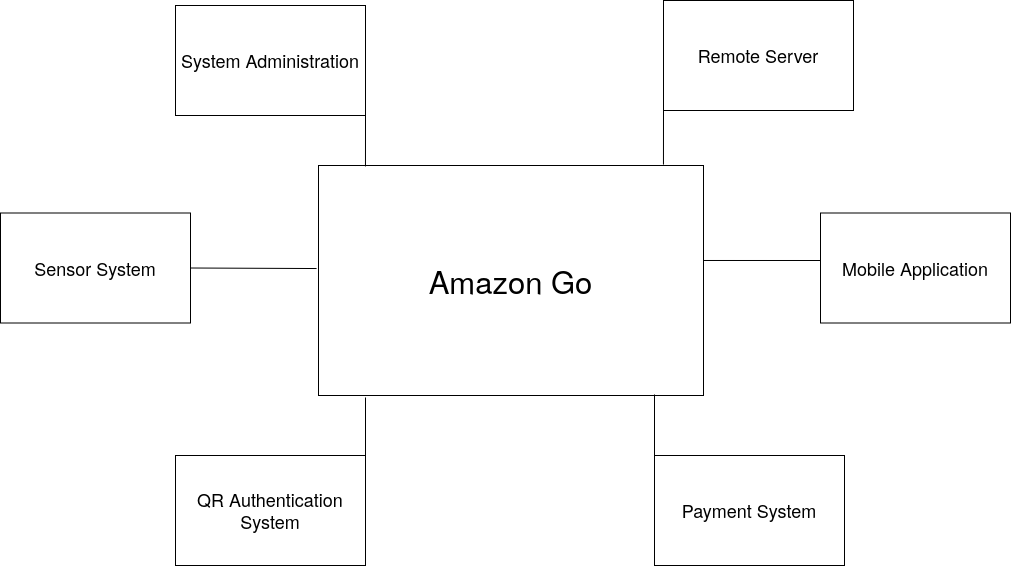
\includegraphics[width=\linewidth]{Images/contextDiagram.png}
            \caption{Context Diagram}
            \label{contextDiagram}
        \end{figure}
        \end{center}

    \begin{center}
        \begin{figure}[H]
            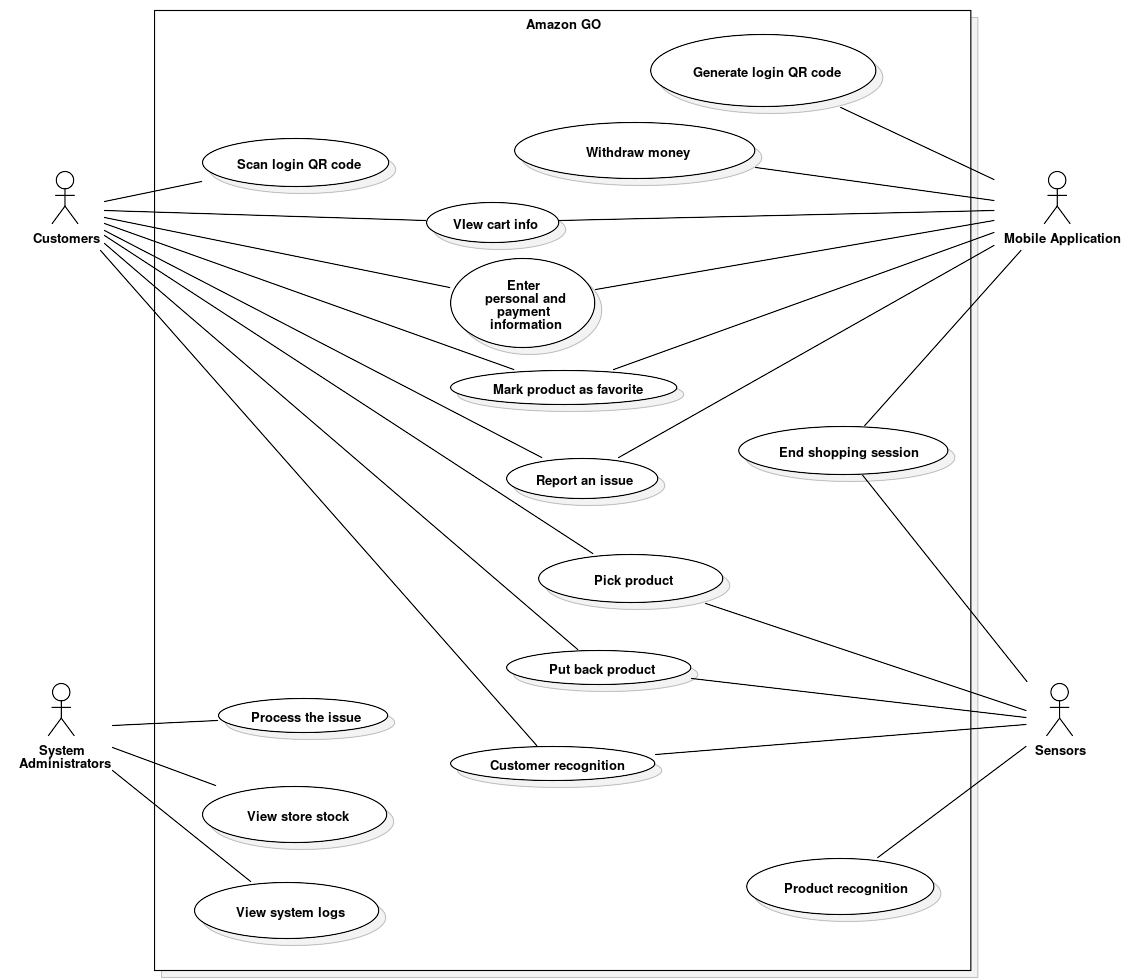
\includegraphics[width=\linewidth]{Images/UseCaseDiagram.png}
            \caption{Use Case Diagram}
            \label{ucaseDiagram}
        \end{figure}
        \end{center}

    \begin{table}[H]
        \begin{centering}
        \begin{tabular}{|p{2.5cm}|p{12cm}|}
        \hline
        Use case name & Customer recognition \\ \hline
        Actors        & Customers, Sensors \\ \hline
        Description   & Immediately after the customer gets his/her QR code scanned, environmental cameras must track his/her movements and positions continuously. Cameras must regularly recognize the customers with their face, clothes etc. and must communicate with the remote server until the customer leaves the store. In order to not to lose visual contact with the customer, every angle in the store must be watched by the cameras and the sensors. \\ \hline
        Data          & Customers' physical details such as clothes, face, and body movements.  \\ \hline
        Stimulus      & The customer getting his/her QR code scanned. \\ \hline
        Response      & Match the user ID with the acquired visual data of the customer. \\ \hline
        Basic Flow    & 
        1- Upon QR scanning, visual sensors receive a user ID and identify the unknown customer with the ID. \newline
        2- Visual sensors track customer's movements and position continuously. \newline
        3- Customer picks up a product. \newline
        4- Customer information is sent to the server.\newline
        5- Flow goes back to step 2. \\ \hline
        Alternative
            Flow \#1  & 
        3- Customer puts a product back to a shelf. \newline
        4- Customer information is sent to the server. \newline
        5- Flow goes back to step 2. \\ \hline
        Alternative
            Flow \#2  &
        3- Customer leaves the store. \newline
        4- Customer information is sent to the server. \newline
        5- System stops tracking the customer. \\ \hline
        Comments      & Immediately after a customer logs in to store, sensors must assign a unique customer ID to that user. \\ \hline
        
        \end{tabular}
        \caption{Customer Recognition}
        \label{tab3}
        \end{centering}
        \end{table}    
        
        
        
        \begin{table}[H]
        \begin{centering}
        \begin{tabular}{|p{2.5cm}|p{12cm}|}
        \hline
        Use case name & Product recognition  \\ \hline
        Actors        & Sensors \\ \hline
        Description   & Right after a product is placed to a shelf by the store staff and the product is marked as 'exist' on the store database, the corresponding ID which belongs to the same product set must be assigned to the product. After that point, until someone buys the product and leaves the store, product must be tracked by using its weight information, visual information, and shelf location. A customer is allowed to take a product, put it into his/her bag, and put the product back to any shelf. In that case, for some time, the visual contact with the product would be lost, but after the product is put back to the shelf, system must recover and continue tracking this product. A customer can put a product back to a different shelf, in that case, the product must be recognized by its visual data and weight again. \\ \hline
        Data          & Weight, physical characteristics, and the location of products. \\ \hline
        Stimulus      & A product is placed to a shelf by the store worker and marked as exist in the store. \\ \hline
        Response      & Match the product with the products in the database. \\ \hline
        Basic Flow    & 
        1- A product is placed to a shelf by the staff. \newline
        2- Query the database with the shelf location, visual data and weight. \newline
        3- Assign the received product ID to corresponding product set.
        \newline
        4- Sensors work continuously to detect product movements. \newline
        5- A product is taken from a shelf. \newline
        6- Product information is sent to the server. \newline
        7- Flow goes back to step 4. \\ \hline
        Alternative
            Flow      & 
        5- A product is placed to a shelf by a customer. \newline
        6- Product information is sent to the server. \newline
        7- Flow goes back to step 4. \\ \hline
        Comments      & Initially, products must be registered to the database and must be assigned to a shelf. \\ \hline
        
        \end{tabular}
        \caption{Product Recognition}
        \label{tab7}
        \end{centering}
        \end{table}    
        

        \begin{table}[H]
        \begin{centering}
        \begin{tabular}{|p{2.5cm}|p{12cm}|}
        \hline
        Use case name & Scan login QR code \\ \hline
        Actors        & Customers \\ \hline
        Description   & A procedure to log users in to store by scanning their QR code via turnstiles. Turnstiles must allow access after a successful scan. Turnstiles must not allow the customers to enter the store if the scan fails and must display the reason. For security reasons, if the same QR is scanned while there is a shopping session with that QR code, login must not be allowed and QR code must be disabled for security purposes. Additionally, customer must be informed about every login with an SMS.    \\  \hline
        Data          & User information. \\ \hline
        Stimulus      & Users showing their QR code to turnstiles. \\ \hline
        Response      & Validation or invalidation of the QR code.  \\ \hline
        Basic Flow    &
        1- Customer shows the QR code to turnstile QR scanner. \newline
        2- Turnstile scans the QR and sends the data to the server. \newline
        3- Server processes the store information and the customer information. \newline
        4- Server responds with success. \newline
        5- Turnstile gives access to the customer. \newline
        6- Server sends SMS notification to the customer. \\ \hline
        Alternative
            Flow      & 
        4- Server responses with failure. \newline
        5- Failure reason is displayed. \newline
        6- Server sends SMS notification to the customer. \\ \hline
        Comments      & Customer must be a registered member. GPS can be used to improve the security.\\ \hline
        
        \end{tabular}
        \caption{Scan Login QR Code}
        \label{tab}
        \end{centering}
        \end{table}    
        
        
                
        \begin{table}[H]
        \begin{centering} 
        
        \begin{tabular}{|p{2.5cm}|p{12cm}|}
        \hline
        Use case name & Pick Product  \\ \hline
        Actors        & Customers, Sensors  \\ \hline
        Description   & A procedure to detect customers when they pick up a product from the shelves. When a customer picks a product, weight sensors must detect the change and must send the related data, also visual sensors must recognize the customer who picks up the product and provide additional data about the product. If the customer picks up multiple products at the same time, sensors must be precise enough to handle the situation.  \\ \hline
        Data          & Customer information, product's price and other information
                        related to that product. \\ \hline
        Stimulus      & Customers picking products. \\ \hline
        Response      & Add the picked product to customer's cart, update the cart information. \\ \hline
        Basic Flow    & 
        1- Customer picks a product up from a shelf. \newline
        2- Weight sensors detect the change. \newline
        3- Visual sensors detect the customer action and assists product recognition. \newline
        4- Sensors send data to server. \newline
        5- Server processes data, adds the related product to customer's cart.
        \\ \hline
        Alternative
            Flow      & - \\ \hline
        Comments      & Customers must get their QR code scanned successfully before shopping. \\ \hline
        
        \end{tabular}
        \caption{Pick Product}
        \label{tab1}
        \end{centering}
        \end{table}    
        
        
        
        \begin{table}[H]
        \begin{centering}
        \begin{tabular}{|p{2.5cm}|p{12cm}|}
        \hline
        
        % uml
        Use case name & Put back product  \\ \hline
        Actors        & Customers, Sensors \\ \hline
        Description   & A procedure to detect customers when they put a product back to shelves. When a customer puts a product back to a shelf, weight sensors must detect the change and must send shelf information, weight information and other related data, also visual sensors must recognize the customer who puts the product back and must provide additional data about the product. System must analyze the cart to be precise about the product. If the customer puts back multiple products at the same time, sensors must be precise enough to handle the situation.\\ \hline
        Data          & Customer information, product's price and other information.  \\ \hline
        Stimulus      & Customers putting a product back to shelf. \\ \hline
        Response      & Delete the related product from the customer's cart. \\ \hline
        Basic Flow    & 
        1- Customer puts a product back to a shelf. \newline
        2- Weight sensors detect the change. \newline
        3- Visual sensors detect the customer action and assists product recognition. \newline
        4- Sensors send data to server. \newline
        5- Server processes data, removes the related product from customer's cart. \\ \hline
        Alternative
            Flow      & - \\ \hline
        Comments      & The product must have been picked up beforehand and this must be in the same session. \\ \hline
        
        \end{tabular}
        \caption{Put Back Product}
        \label{tab2}
        
        \end{centering}
        \end{table}    
        
        
                
        \begin{table}[H]
        \begin{centering}
        \begin{tabular}{|p{2.5cm}|p{12cm}|}
        \hline
        Use case name & View cart info  \\ \hline
        Actors        & Customers, Mobile Application \\ \hline
        Description   & A customer must be able to see it's current cart status 
                        by using the mobile app. Customer shall see the products she/he picked up, with their quantity and price. Total price must be also displayed. \\ \hline
        Data          & The customer's cart status. \\ \hline
        Stimulus      & The customer pressing the 'My Cart' button on the app.  \\ \hline
        Response      & Show the customer's current cart status.  \\ \hline
        Basic Flow    & 
        1- Customer opens the app. \newline
        2- Customer logins if not signed in already. \newline
        3- Application opens the cart screen automatically. \newline
        4- Application sends view cart request to the server. \newline
        5- Server responds with the related data. \newline
        6- Application shows the cart status. \\ \hline
        Alternative
            Flow      & - \\ \hline
        Comments      & Data must be fetched from the remote server in case of an attempt to cheat. User must be shopping to be able to see the cart screen.\\ \hline
        
        \end{tabular}
        \caption{View Cart Info.}
        \label{tab4}
        \end{centering}
        \end{table}    
        
        
        
        \begin{table}[H]
        \begin{centering}        
        \begin{tabular}{|p{2.5cm}|p{12cm}|}
        \hline
        Use case name & Enter personal and payment information  \\ \hline
        Actors        & Customers, Mobile Application  \\ \hline
        Description   & When a customer signs up, s/he must provide personal 
                        information and payment method. If the payment method is invalid, application must request a valid method and must not allow another action to be taken by the customer until a valid payment method is provided.  \\ \hline
        Data          & Personal data and payment data.  \\ \hline
        Stimulus      & When a customer signs up or updates his/her information. \\ \hline
        Response      & Validation or invalidation of the payment method. If validated, sign up or update the user. \\ \hline
        Basic Flow    & 
        1- Application shows a personal information form or a payment form. \newline
        2- User enters information. \newline
        3- Application checks the validity of the information at the same time. \newline
        4- If everything is valid, a button is enabled to finish the process. \newline
        5- User presses the button. \newline
        6- Server inserts the related information to the database. \\ \hline
        Alternative
            Flow      & - \\ \hline
        Comments      & If the customer is a member, then instead of signing him/her up, update the information. \\ \hline
        
        \end{tabular}
        \caption{Enter Personal and Payment Information}
        \label{tab5}
        \end{centering}
        \end{table}    
        
        
        
        \begin{table}[H]
        \begin{centering}        
        \begin{tabular}{|p{2.5cm}|p{12cm}|}
        \hline
        Use case name & End shopping session  \\ \hline
        Actors        & Mobile Application, Sensors \\ \hline
        Description   & Visual sensors must detect when the customer leaves the store and report to remote server. Details about the shopping session must be visible from the application after session ends.  \\ \hline
        Data          & Customer ID, store information.  \\ \hline
        Stimulus      & Customer leaving the store. \\ \hline
        Response      & Session information. \\ \hline
        Basic Flow    & 
        1- Customer walks out from the store. \newline
        2- Visual sensors detects the action. \newline
        3- End shopping session request is sent to servers with the customer ID. \newline
        4- Server processes the request and saves the sessions information to the database. \newline
        5- Visual sensors stop tracking that customer. \\ \hline
        Alternative
            Flow      & - \\ \hline
        Comments      & Log the current session to database for possible further use.  \\ \hline
        
        \end{tabular}
        \caption{End Shopping Session}
        \label{tab6}
        \end{centering}
        \end{table}    
        
        
                
        \begin{table}[H]
        \begin{centering}
        \begin{tabular}{|p{2.5cm}|p{12cm}|}
        \hline
        Use case name & Generate login QR code \\ \hline
        Actors        & Mobile Application \\ \hline
        Description   & Application must generate a unique QR code to enable customers log in. A generated QR code can be used multiple times until it is disabled due to security or user prompt. QR codes must be user specific. \\ \hline
        Data          & Customer information. \\ \hline
        Stimulus      & User pressing the 'QR Code' button on the mobile app. \\ \hline
        Response      & Produce and show the QR code \\ \hline
        Basic Flow    & 
        1- A customer signs up. \newline
        2- Application requests a QR code for the customer. \newline
        3- Server generates a QR code that is unique to the customer.\\ \hline
        Alternative
            Flow      &
        1- Customer presses the Refresh QR button. \newline
        2- Application requests a QR code for the customer. \newline
        3- Server generates a QR code that is unique to the customer.\\ \hline
        Comments      & QR code must be generated and sent by the remote server in case of a cheating attempt. \\ \hline
        
        \end{tabular}
        \caption{Generate Login QR Code}
        \label{tab8}
        \end{centering}
        \end{table}    
        
        
                
        \begin{table}[H]
        \begin{centering}
        \begin{tabular}{|p{2.5cm}|p{12cm}|}
        \hline
        Use case name & Withdraw money \\ \hline
        Actors        & Mobile Application \\ \hline
        Description   & When user leaves the store, withdraw money from his/her registered payment method. System must use the payment method provided by the customer. If the payment attempt fails due to lack of money or other reasons, notifications must be sent regularly until customer pays. Customer must not be allowed to shop until she/he pays.    \\ \hline
        Data          & User ID. \\ \hline
        Stimulus      & Upon the 'End shopping session' procedure. \\ \hline
        Response      & Confirmation that payment is successful.  \\ \hline
        Basic Flow    & 
        1- System is informed by the End Shopping Session function. \newline
        2- System requests a payment from the user's payment method via the Payment API. \newline
        3- Payment is successful. \newline
        4- Receipt is created.  \\ \hline
        Alternative
            Flow      & 
        3- Payment is failed. \newline
        4- An SMS notification is sent to the customer. \newline
        5- The customer is blacklisted until the she/he pays. \\ \hline
        Comments      & Further actions can be taken by the authorities if a payment is not received for a long time. \\ \hline
        
        \end{tabular}
        \caption{Withdraw Money}
        \label{tab9}
        \end{centering}
        \end{table}    
        
        
                
        \begin{table}[H]
        \begin{centering}
        \begin{tabular}{|p{2.5cm}|p{12cm}|}
        \hline
        Use case name & View store stock  \\ \hline
        Actors        & System Administrator \\ \hline
        Description   & System admins must be able to see current stock status of each store and main warehouse. User must be warned about low stocks.\\ \hline
        Data          & Store ID, admin ID. \\ \hline
        Stimulus      & User pressing the 'View Stock' button on the mobile app. \\ \hline
        Response      & Stock information .\\ \hline
        Basic Flow    &
        1- System admin opens the administration page. \newline
        2- User presses the stock status tab. \newline
        3- Overall stock status of each store is listed to the user. Stocks are colored according to the amount. \newline
        4- User selects a store. \newline
        5- Detailed stock status of the selected store is shown to the user.
        \\ \hline
        Alternative
            Flow      & - \\ \hline
        Comments      & User must be authorized to view stock information. \\ \hline
        \end{tabular}
        \caption{ View Store Stock }
        \label{tab_10}
        \end{centering}
        \end{table}    
        
        
                
        \begin{table}[H]
        \begin{centering}
        \begin{tabular}{|p{2.5cm}|p{12cm}|}
        \hline
        Use case name & View system logs  \\ \hline
        Actors        & System Administrators \\ \hline
        Description   & Administrators must be able to see previous shopping session details of customers. Any inconsistency in sessions must be reported. \\ \hline
        Data          & Time and date, Store ID, Customer ID \\ \hline
        Stimulus      & Administrators reaching the log files. \\ \hline
        Response      & Previous cart information, payment method  \\ \hline
        Basic Flow    & 
        1- System admin opens the administration page. \newline
        2- User presses the view logs tab. \newline
        3- Several filter options are shown to the user. \newline
        4- User fills some of the filtering fields. \newline
        5- User presses the search button. \newline
        6- Results are listed. \\ \hline
        Alternative
            Flow      & - \\ \hline
        Comments      & Only administrators can see the log files. \\ \hline
        \end{tabular}
        \caption{View System Logs}
        \label{tab_11}
        \end{centering}
        \end{table}    

        %% == NEW USES CASES == %%
        \begin{table}[H]
            \begin{centering}
            \begin{tabular}{|p{2.5cm}|p{12cm}|}
            \hline
            Use case name & Mark Product as Favorite \\ \hline
            Actors        & Customers, Mobile Application \\ \hline
            Description   & Customers should be able to add a product that they buy frequently or a product that they wish to buy to their favorite products list. \\ \hline
            Data          & Product ID, Customer ID \\ \hline
            Stimulus      & A user pressing the 'Star' on the page of the product using the mobile application. \\ \hline
            Response      & A message indicating whether the operation was successful or not.  \\ \hline
            Basic Flow    & 
            1- Customer logs in to the mobile application. \newline
            2- User navigates to the product's page on the mobile application via the search button or via the categories. \newline
            3- System loads the product page. \newline
            4- User presses the dimmed 'Star' icon on the loaded page. \newline
            5- 'Star' icon is lighted up and the product is added to the user's favorites. \\ \hline
            Alternative
                Flow      & 
                4- User presses the already lighted up 'Star' icon \newline
                5- 'Star' icon is dimmed and the product is removed from the user's favorites. \\ \hline
                
            Comments      & On each press to 'Star' icon, the icon is basically toggled. \\ \hline
        \end{tabular}
        \caption{Mark Product as Favorite}
        \label{tab_12}
        \end{centering}
        \end{table}    

        \begin{table}[H]
            \begin{centering}
            \begin{tabular}{|p{2.5cm}|p{12cm}|}
            \hline
            Use case name & Report an Issue  \\ \hline
            Actors        & Customers, Mobile Application \\ \hline
            Description   & A user should be able to communicate with the system admins in case of any problems or questions.\\ \hline
            Data          & User ID, User Message \\ \hline
            Stimulus      & User presses the 'Report an Issue' button at the main page of the mobile application. \\ \hline
            Response      & Validation that issue is reported or not.  \\ \hline
            Basic Flow    & 
            1- Customer logs in to the mobile application. \newline
            2- User navigates to the issue reporting page by pressing the 'Report an Issue' button. \newline
            3- A textbox appears on the screen which waits for user to enter his message.\newline
            4- User enters his/her message and presses the send button. \newline
            5- A notification appears if the message is transmitted successfully or not. \\ \hline
            Alternative
                Flow      & - \\ \hline
            Comments      & If a user sends two seperate messages consecutively, these messages shall be merged to avoid spam. Also a user 
                            should be able to send only one message in ten minutes. \\ \hline
        \end{tabular}
        \caption{Report an Issue}
        \label{tab_13}
        \end{centering}
        \end{table}    


        \begin{table}[H]
            \begin{centering}
            \begin{tabular}{|p{2.5cm}|p{12cm}|}
            \hline
            Use case name & Process the Issue  \\ \hline
            Actors        & System Administrators \\ \hline
            Description   & System admins inspect the issue provided by the user and take action accordingly. \\ \hline
            Data          & Response Message, User ID \\ \hline
            Stimulus      & An admin pressing the 'Inspect Issues' button on the admin page and selecting an issue.\\ \hline
            Response      & The status of the selected issue is updated (such as ongoing, solved etc.) \\ \hline
            Basic Flow    & 
            1- An admin logs into the admin page using his Admin ID and password. \newline
            2- The admin presses the 'Inspect Issues' button on the admin page.\newline
            3- A list of unsolved issues are shown to the admin.  \newline
            4- The admin selects an issue by the date (early messages first). \newline
            5- The admin takes action (such as inspecting the logs) and sends a reply to the issuer. \\ \hline
            Alternative
                Flow      & 
            6- The admin marks the issue as solved.\\ \hline
            Comments      & \\ \hline
        \end{tabular}
        \caption{Process the Issue}
        \label{tab_14}
        \end{centering}
        \end{table}    



    \subsection{Composition View}
        In this viewpoint, the components of the system are shown from a top-level point of view. Also, the design rationale for 
        each decision is provided right after the \nameref{componentDia}. 


        \begin{center}
            \begin{figure}[H]
                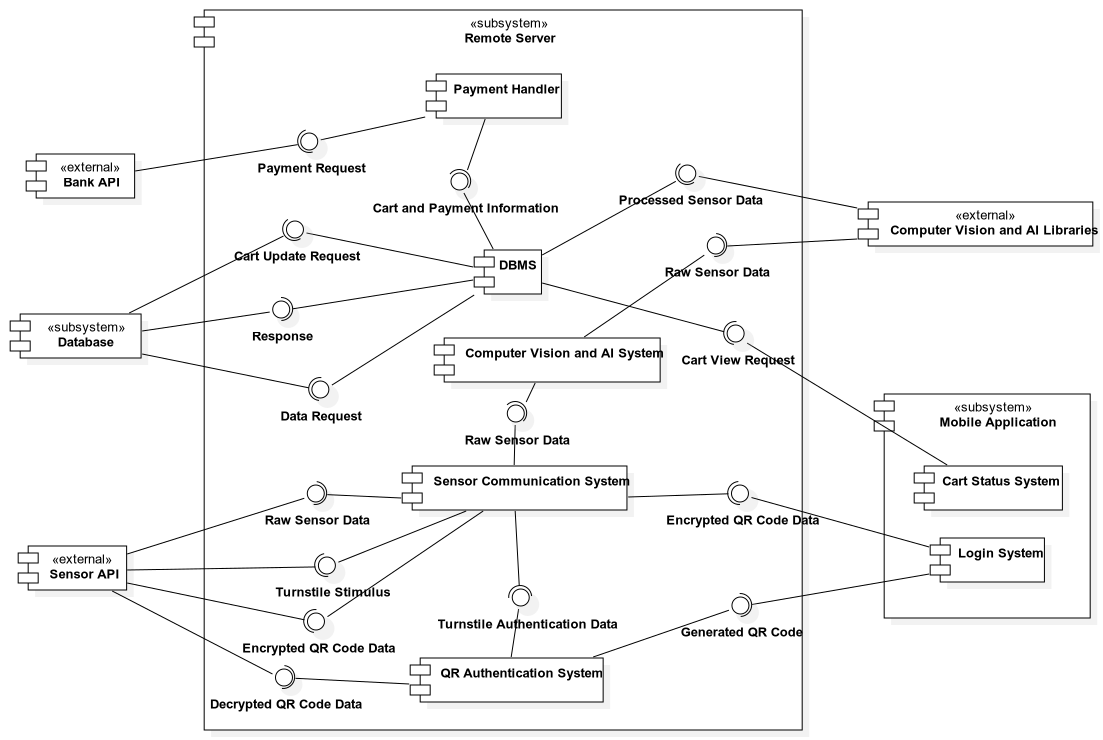
\includegraphics[width=\linewidth]{Images/ComponentDiagram.png}
                \caption{Component Diagram}
                \label{componentDia}
            \end{figure}
        \end{center}

    \textbf{Design Rationale: \\}
    \begin{itemize}
        
        \item Remote Server is the component where most of the things are done. Any communication between components, interaction with database and any calculation 
        that needs to be done for the AI and Computer Vision algorithms are done on the remote server.
        
        \item AI and Computer Vision calculations are done via the libraries, which reside on the server.
        
        \item Amazon Go is a system that needs to handle several different tasks at the same time. Some of these tasks follow similar routines.
        Therefore some generic components and interfaces like Sensor Communication system are used, which allows to keep the diagram simple
        and more understandable.

        \item QR Authentication System is basically the entrance point of the system. It produces the QR code, then forwards it to the Login System of the mobile 
        application. Then, the user gets his/her QR code scanned by the turnstiles, which posts the encrypted QR code to Sensor Communucation System. Sensor 
        Communication System forwards this data to the corresponding Sensor API, QR code gets decrypted, and sent back to the QR Authentication System. 
        QR Authentication system either validates or invalidates the QR Code, and depending on the output, it sends information to Sensor Communucation System, 
        which then may send a stimulus for the turnstiles depending on the validation output.
        
        \item Sensor Communication System is used as an abstraction to define communication of all kinds of sensors including cameras, QR scanners on turnstiles 
        and weight sensors on shelves. Raw sensor data is the sensor data produced by the corresponding sensor. This might be image data or weight data. 
        QR Code data is shown separately as it has a separate target component.
        
        \item Computer Vision and AI System is basically a bridge between the Sensor Communication System and Computer Vision and AI Libraries. Any raw data that is 
        produced by the sensors first passes through Sensor Communication System, which forwards this raw data to Computer Vision and AI System, which then 
        forwards this data to the required libraries to be processed.
        
        \item DBMS is the place where the interaction with the database and the manipulation of the database take place. 
        
        \item Payment Handler is a component which is responsible of the payments. When a user exits the store, required payment information is taken from the 
        database via DBMS, and this data is forwarded to Payment Handler. Depending on the bank, Payment Handler makes calls to the corresponding Bank API. 
        
        \item Mobile application provides some functionalities for the end users. It must communicate with the remote server in order to provide QR authentication and 
        cart view features.
        
        \item Database mostly holds user and product related information. These data might be customers' and products' physical properties, customers' name, products' 
        price and etc. Computer vision and AI mostly depend on that information while operating.
        
        \item Bank API is an abstraction that is used to define different Bank APIs. Depending on the user's choice of bank, it uses a different bank's API.
    \end{itemize}

    \begin{center}
        \begin{figure}[H]
            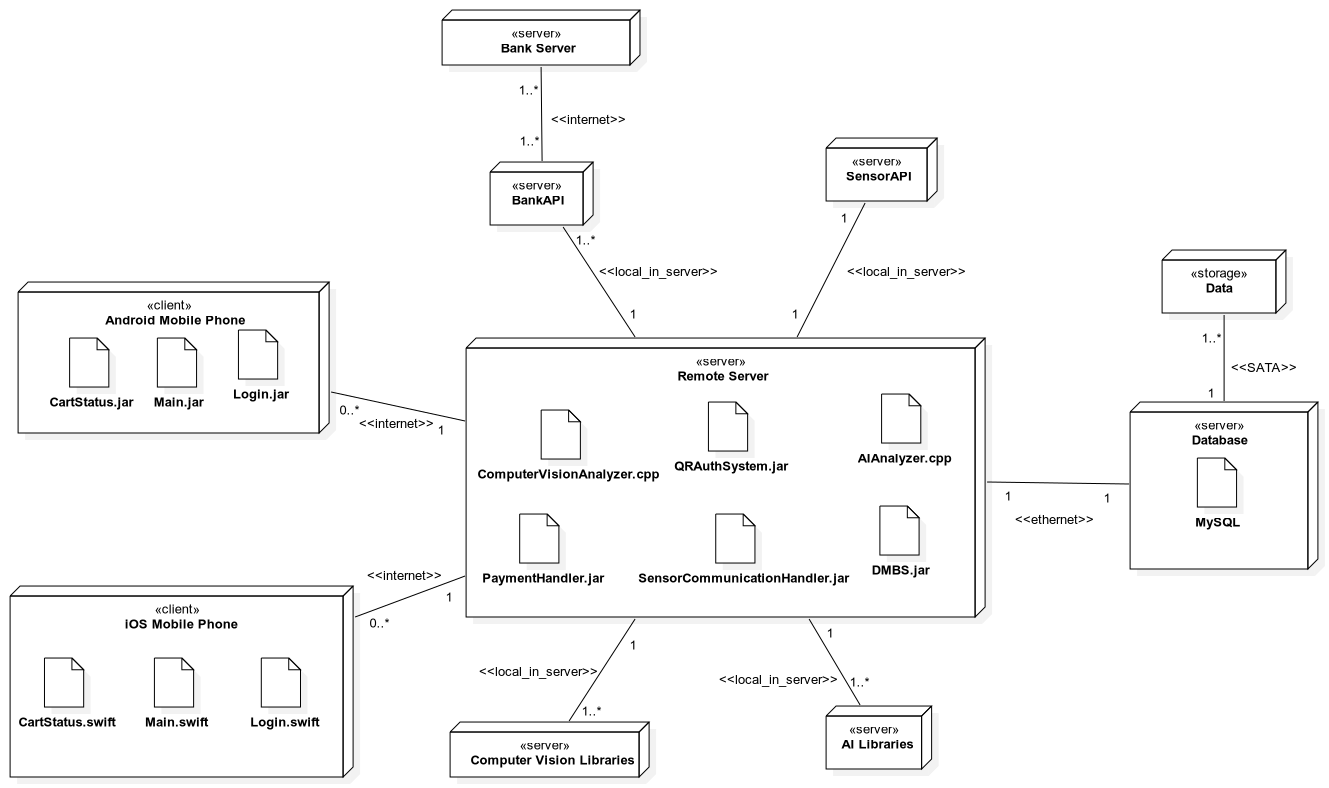
\includegraphics[width=\linewidth]{Images/DeploymentDiagram.png}
            \caption{Deployment Diagram}
            \label{deployDia}
        \end{figure}
    \end{center}
    
    \textbf{Design Rationale: \\}
    \begin{itemize}
        \item The database is separate from the remote server so that in case of a system failure, the data does not get corrupted.
        
        \item Storage devices that are used in the database are connected via SATA interface as HDDs will be used as storage devices since SSDs are
        too expensive to use as storage. 
        
        \item There are two mobile applications, one for Android and one for iOS. These will be downloadable from the corresponding stores. Main.jar and Main.swift 
        are shown to show that these mobile applications will be developed in Java and Swift, respectively.
        
        \item The connections that are represented by $<<local\_in\_server>>$ means that these parts reside on the same computer that acts as a server. In other words,
        they are basically stored in the storage devices of the server, which can be accessed by a basic disk seek operation.

        \item MySQL is used for DBMS since it is open source and free.
        
        \item For simplicity, only one storage device which is connected to database is shown. However, system will use more than one storage devices, and some of them
        will be used as backup disks.

    \end{itemize}

    
    \subsection{Information View}
    In this view, the organization and the relations of the data in the database and their class counterparts, methods and attributes of these classes are shown. 
    Detailed information about the operations are given after the \nameref{icd}. Furthermore, classes that are needed by the database operations can be seen 
    in detail on the Database Class Diagram. %NAMEREF HERE
    
    \subsubsection{Interfaces}
    \begin{center}
        \begin{figure}[H]
            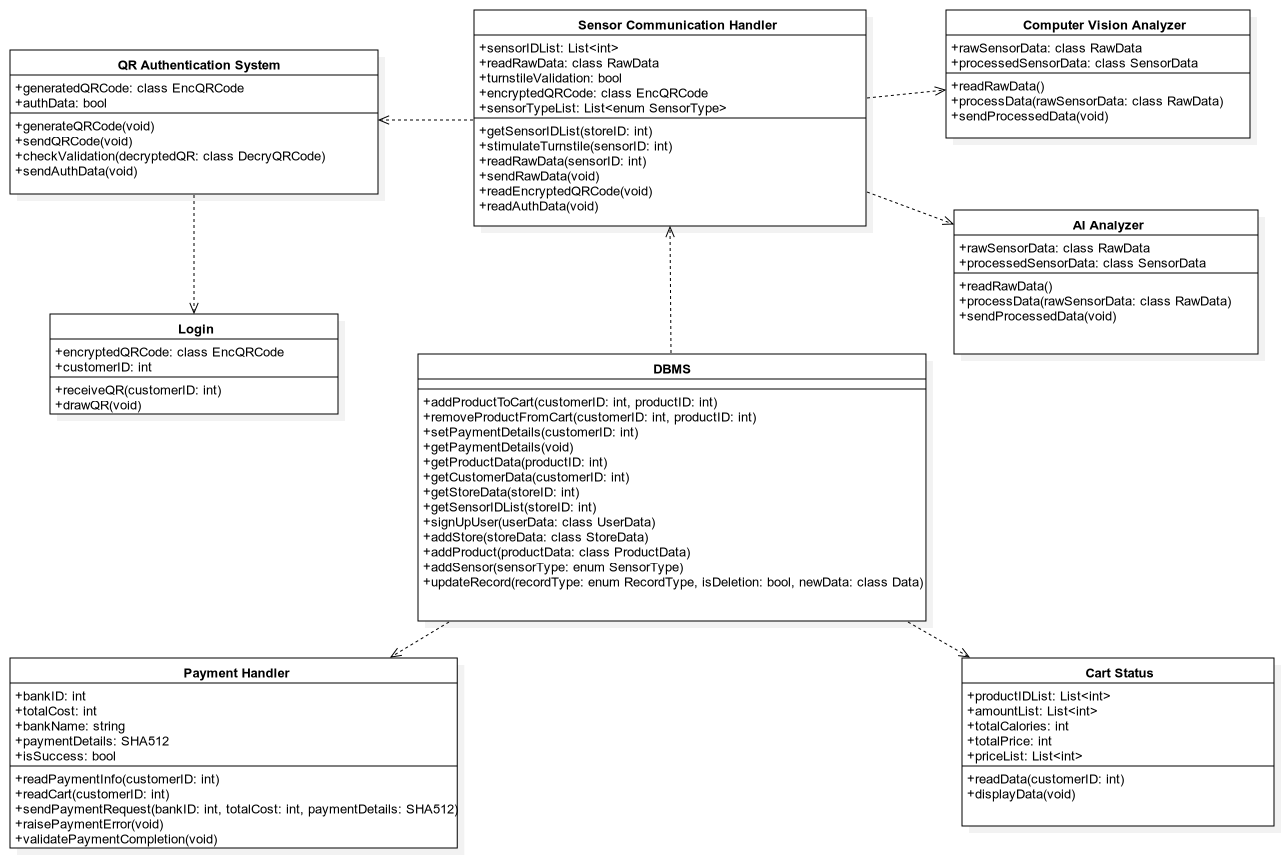
\includegraphics[width=\linewidth]{Images/InterfaceClassDiagram.png}
            \caption{Interface Class Diagram}
            \label{icd}
        \end{figure}
    \end{center}

    \begin{longtable}[H]{|p{5cm}|p{11cm}|}
        \hline
        \textbf{Operation} & \textbf{Description} \\ \hline
        generateQRCode & Generates a QR code for authentication. \\ \hline
        sendQRCode & Sends the generated QR code to the mobile app. \\ \hline
        checkValidation & Takes the decrypted QR code as input and checks whether it is valid or not. \\ \hline
        sendAuthData & Sends the validation that is obtained from the checkValidation to the Sensor Communication System. \\ \hline
        drawQR & Draws the generated QR Code onto the screen of the user's mobile application.\\ \hline
        readPaymentInfo & Gets the payment information of the given customer by making calls to related Database Handler getter functions.\\ \hline
        readCart & Gets the current cart information of the given customer by making calls to related Database Handler getter functions.\\ \hline
        sendPaymentRequest & Chooses the correct Bank API and sends a request to this API to make the payment.\\ \hline
        raisePaymentError & If payment is not successful, displays an error message. \\ \hline
        validatePaymentCompletion & If payment is successful, displays a success message.\\ \hline
        getSensorIdList & Given storeID, retrieves all sensors in this store and writes it to its sensorIDList variable.\\ \hline
        stimulateTurnstile & If the validation of QR code is successful, sends a stimulant to turnstiles to open them.\\ \hline
        readRawData & Reads the raw data (not processed data) from the sensors onto rawData variable. \\ \hline
        sendRawData & Forwards rawData variable to AI Analyzer and Computer Vision Analyzer.\\ \hline
        readEncryptedQRCode & After the QR code is generated and displayed on the user end, this function is called to obtain the generated QR code.\\ \hline
        processData & Makes required computations for Computer Vision and AI.\\ \hline       
        sendProcessedData & Posts the output of computations that are done by Computer Vision and AI to database handler to be registered.\\ \hline
        readData & Retrieves the given customer's cart data by communicating with database handler..\\ \hline
        displayData & Displays the retrieved cart data on the user's mobile app. \\ \hline
        updateRecord & Updates the given record on the corresponding table. Class Data is a base class which instantiates other data classes 
        such as class CustomerData, class StoreData etc.\\ \hline
        addRecordToTable & Inserts the given record to the corresponding table.\\ \hline
        deleteRecordFromTable & Deletes the given record from the corresponding table by ID.\\ \hline
        getPaymentDetails & Gets the payment details of the given customer from the database.  \\ \hline
        getProductData & Gets the product information of the given product from the database. \\ \hline
        getCustomerData & Gets the customer information of the given customer from the database. \\ \hline      
        getStoreData & Gets the store information of the given store from the database. \\ \hline
        getSensorIdList & Gets all the sensors' ID that are in the given store from the database. \\ \hline
        authorizeStoreWorker & Adds a store worker to the given storeID. Used when employing a store worker. \\ \hline
        readReceipt & Gets the receipt data according to given parameters from the database. \\ \hline
        readLog & Gets the logs that are related to given parameters from the database. \\ \hline
        getCurrentCart & Gets the given customer's current cart information from the database. \\ \hline  
    \caption{Operation Descriptions}
    \label{oper_desc}
    \end{longtable}       
    
    \textbf{Important Note:} The table below is the Operation Design Table. Some of the entries' input field are denoted with void, however since this is an object oriented paradigm design, these methods may use its class' local variables. Hence, please refer to \nameref{icd} in order to see what local variables are used for void input fields.\\
    
    \begin{longtable}[H]{|p{3.8cm}|p{3cm}|p{4cm}|p{4.5cm}|}
        \hline
        \textbf{Operation} & \textbf{Inputs} & \textbf{Outputs} & \textbf{Exceptions} \\ \hline
        generateQRCode 
        & void 
        & Returns the generated QR Code.  
        & - \\ \hline
        
        sendQRCode
        & -targetCustomerID
        & Sends the generated QR Code to the user with the ID targetCustomerID. 
        & targetCustomerID 
        is not a valid user or connection with the target customer is lost.  \\ \hline
        
        checkValidation
        & -decryptedQR 
        & Returns true if the decrypted QR code is valid.
        & Checksum of the decrypted QR code differs(data loss in transmission) or decrypted QR code is NULL.  \\ \hline
       
        sendAuthData 
        & void 
        & Returns the message sent to the Sensor Communication System. 
        & Sensor Comm. System is busy or connection error occurs. \\ \hline
        
        
        drawQR 
        & void 
        & Returns true if the encryptedQRCode variable is successfully drawn.
        & Database connection error occurs or encryptedQRCode is NULL.\\ \hline
        
        readPaymentInfo 
        & -customerID
        & Returns all the defined payment information of the customer with the ID customerID.
        & customerID is not a valid or database connection error occurs.\\ \hline
       
        readCart 
        & -customerID 
        & Returns the current cart information of the customer with the ID customerID.
        & customerID is not a valid or database connection error occurs. \\ \hline
       
        sendPaymentRequest 
        & -bankID \makecell{-totalCost} -paymentDetails
        & Returns true if the request results in success.
        & bankID or paymentDetails are not valid or database connection error occurs.\\ \hline
       
        raisePaymentError
        & void
        & Prints an error message indicating that payment has failed.
        & sendPaymentRequest function throws an exception or connection with the user is lost.\\ \hline
       
        validatePayment
       
        Completion 
        & void
        & Prints a success message indicating that payment is a success. 
        & sendPaymentRequest function throws an exception or connection with the user is lost.\\ \hline
       
        getSensorIdList 
        & -storeID
        & Given storeID, returns all list of sensors in this store.
        & storeID is not valid or retrieved list is NULL or database connection occurs.\\ \hline
       
        stimulateTurnstile 
        & -sensorID
        & Signals the turnstile with the sensorID and returns true.
        & sensorID is not valid or sensor with the given sensorID is not a turnstile or the turnstile is offline.\\ \hline
       
        readRawData 
        &-sensorID  
        & Returns the read raw data from the sensors.
        & sensorID is not valid or sensor with the given sensorID is not a turnstile or the turnstile is offline or raw data is NULL.\\ \hline
       
        sendRawData 
        & void
        & Returns true if the forwarding of the rawData variable is complete.
        & rawData is NULL or Computer Vision-AI system is overworking hence losing performance.\\ \hline
       
        readEncryptedQRCode 
        & void
        & Returns the encrypted QR code that is read from the user. 
        & Read QR code is NULL or connection with the user is lost.\\ \hline
       
        processData 
        & -rawSensorData
        & Returns the Computer Vision and AI processing results obtained processing the rawSensorData.
        & rawSensorData is NULL or Computer Vision-AI system is overworking.\\ \hline    
       
        sendProcessedData 
        & void
        & Returns true if the processedData variable is successfully registered in the database.
        & processedData is NULL or database connection error occurs.\\ \hline
       
        readData 
        & -customerID
        & Returns the read current cart information of the given user.
        & Connection with the database is lost or user is not logged in or customerID is not valid.\\ \hline
       
        displayData 
        & void
        & Displays the current cart information using the class' local variables and returns true on success.
        & Data to be displayed is NULL.\\ \hline
       
        updateRecord 
        & -tableTypeID \makecell{-newData} -searchedData
        & Returns true if the update is successful, else false. 
        & tableTypeID is not a valid table ID or searchedData is not found or connection with the database is lost.\\ \hline
        
        addRecordToTable 
        & -tableTypeID \makecell{-addedData}
        & Returns true if the addition is successful, else false.
        & tableTypeID is not a valid table ID or addedData is NULL or connection with the database is lost.\\ \hline
       
        deleteRecordFromTable 
        & -tableTypeID \makecell{searchedRecord}
        & Returns true if the deletion of the searchedRecord is successful.
        & searchedRecord is NULL or tableTypeID is not valid or connection with the databse is lost.\\ \hline
        
        getPaymentDetails 
        & -customerID \makecell{-type}
        & Returns the payment details of the given customerID specified with type.
        & customerID is not valid or type is not an accepted payment method or database connection error occurs.\\ \hline
        
        getProductData
        & -productID
        & Returns the all data related to given productID from the database.
        & productID is not valid or connection with the database is lost.\\ \hline
        
        getCustomerData 
        & -customerID
        & Returns customer information of the customer with ID customerID from the database. 
        & customerID is not valid or database connection error occurs.\\ \hline      
        
        getStoreData 
        & -storeID
        & Returns all the information of the store with the ID storeID from the database.
        & storeID is not valid or database connection is lost.\\ \hline
        
        getSensorIdList
        & -storeID
        & Returns the all list of sensors in the given storeID from the database.
        & storeID is not valid or database connection is lost.\\ \hline
        
        authorizeStoreWorker 
        & -storeID \makecell{-storeWorkerData}
        & Returns true if the authorization of the new worker is successful.
        & storeID is not valid or storeWorkerData is NULL or database connection error occurs.\\ \hline
        
        
        readReceipt 
        & -receiptID \makecell{-cartID} -storeID
            \makecell{-customerID} \makecell{-paymMethod}
        & Returns the receipt information of the given user in the given store with the given payment method and cartID from the database.
        & At least one of the given parameters is invalid or database connection error occurs.\\ \hline
        
        readLog 
        & -logNumber \makecell{-customerID} -productID \makecell{-storeID}
        & Returns the log that are associated with the given parameters from the database.
        & At least one of the given parameters is invalid or database connection error occurs.\\ \hline
        
        getCurrentCart 
        & -customerID
        & Returns the current cart information of the given user.
        & customerID is not valid or customer is not logged in (i.e not shopping currently) or database connection error occurs.\\ \hline  
        
        \caption{Operation Design }

    \label{oper_design}
    \end{longtable} 
     

 

    \textbf{Design Rationale:\\}
    \begin{itemize}
        
        \item There is a base class called class Data, which basically forms a base for all the class items that are stored in the database such as customer information, store information etc.
        
        \item By doing so, we do not have to write different methods or a method with lots of if-switch statements in the Database Handler for each data type update or delete. We can directly call these methods with this class Data and depending on the tableTypeID, it makes the corresponding changes on this table.
       
        \item By avoiding these if-switch statements and extra methods, we increase both the performance of the database operations and maintainability of the code.
        
        \item All methods that use a class as its input throws an exception if the class data is NULL so that no NULL data is stored in the database. This increases the speed of the database and reduces the storage needed for the database. 
        
        \item Depending on some special days such as Black Friday, number of customers may increase, which in turn puts lots of pressure on the Computer Vision and AI System. 
        If that is the case and we keep loading more data on them, it may crash the system or may produce corrupt data. To prevent this, System Communication Handler may choose to buffer rawData rather than immediately sending it to the Computer Vision and AI libraries.
        \item All systems are directly or indirectly connected to Database Handler since Amazon Go is based on a data processing system. Hence, Database Handler is basically the "main" of the Amazon Go.
        
        \item Since this is an object oriented paradigm design, some functions do not take parameters. For further information about void input, please read the \textbf{Important Note} that is placed right before the \nameref{oper_design} Table.
    \end{itemize}
    
    \subsubsection{Database Operations}

    \begin{center}
        \begin{figure}[H]
            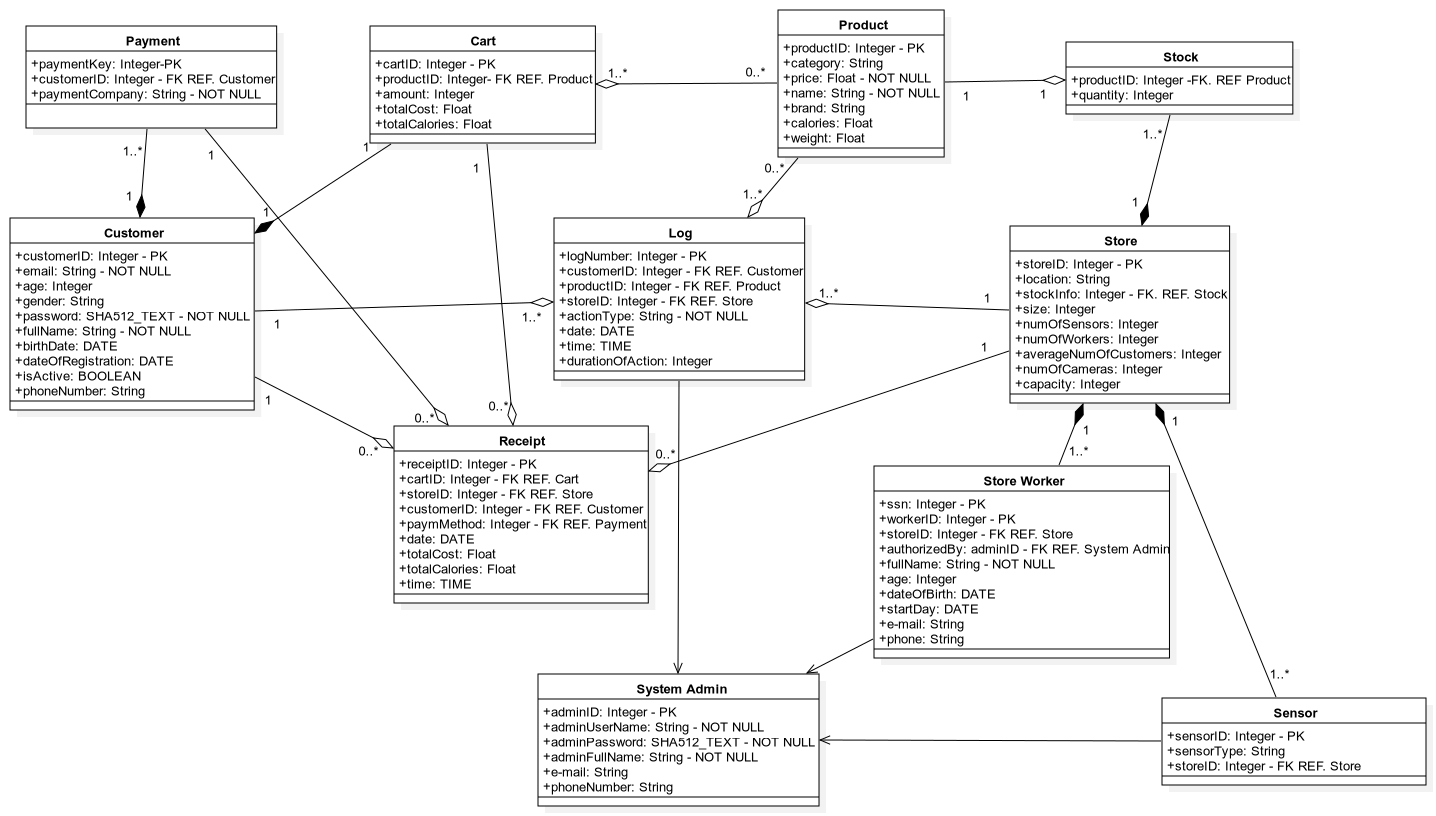
\includegraphics[width=\linewidth]{Images/DatabaseClassDiagram.png}
            \caption{Database Class Diagram}
            \label{dcd}
        \end{figure}
    \end{center}

    \begin{longtable}[H]{|p{5cm}|p{9cm}|}
        \hline
        \textbf{Operation} & \textbf{CRUD} \\ \hline
        generateQRCode & 
          Create: Log \newline
          Read  : Customer \newline
          Update: \newline
          Delete: \\ \hline
        readPaymentInfo & 
          Create: \newline
          Read  : Payment \newline
          Update: \newline
          Delete: \\ \hline
        readCart & 
          Create: \newline
          Read  : Customer, Cart \newline
          Update: \newline
          Delete: \\ \hline
        validatePaymentCompletion & 
          Create: Receipt, Log \newline
          Read  : \newline
          Update: \newline
          Delete: Cart \\ \hline
        sendProcessedData & 
          Create: Log \newline
          Read  : \newline
          Update: Cart \newline
          Delete: \\ \hline
        updateRecord & 
          Create: Log \newline
          Read  : \newline
          Update: Payment, Customer, Cart, Product, Stock, Store, Store Worker, Sensor, System Admin \newline
          Delete: \\ \hline
        addRecordToTable & 
          Create: Payment, Customer, Cart, Product, Stock, Store, Store Worker, Sensor, System Admin, Receipt, Log \newline
          Read  :  \newline
          Update: \newline
          Delete: \\ \hline
        deleteRecordFromTable & 
          Create: Log \newline
          Read  : \newline
          Update: \newline
          Delete: Payment, Customer, Cart, Product, Stock, Store, Store Worker, Sensor, System Admin \\ \hline
        getPaymentDetails & 
          Create: \newline
          Read  : Payment \newline
          Update: \newline
          Delete: \\ \hline
        getCustomerData & 
          Create: \newline
          Read  : Customer \newline
          Update: \newline
          Delete: \\ \hline
        getStoreData & 
          Create: \newline
          Read  : Store \newline
          Update: \newline
          Delete: \\ \hline
        getSensorIDList & 
          Create: \newline
          Read  : Sensor \newline
          Update: \newline
          Delete: \\ \hline
        authorizeStoreWorker & 
          Create: Store Worker, Log \newline
          Read  : \newline
          Update: \newline
          Delete: \\ \hline
        readReceipt & 
          Create: \newline
          Read  : Receipt \newline
          Update: \newline
          Delete: \\ \hline
        readLog & 
          Create: \newline
          Read  : Log \newline
          Update: \newline
          Delete: \\ \hline
        getCurrentCart & 
          Create: \newline
          Read  : Cart \newline
          Update: \newline
          Delete: \\ \hline
        
    \caption{CRUD Operations}
    \label{CRUD}
    \end{longtable}       


    \textbf{Design Rationale:\\}
    \begin{itemize}
        \item MySQL will be used as the database management system.
        \item Important operations will create logs as it can be seen on the \hyperref[CRUD]{Table 18.}
        \item updateRecord, addRecordToTable and deleteRecordFromTable are generic functions that are able to manipulate certain tables. These will also create a log every time they are called.
    \end{itemize}


    \subsection{Interface View}
    In this view, the internal interfaces between the components of the system and the external interfaces between the 
    Amazon Go and the other systems will be specified in detail.

    
    \subsubsection{Internal Interfaces}
    \textbf{The Interface between the Database Handler and the Sensor Communication Handler:\\}
    Database Handler uses Sensor Communication Handler in order to send data to sensors and receive data from the sensors. Information that need to be stored are first passes
    through Sensor Communication Handler, and stop at Database Handler in order to be stored. When the data needs to be processed, Database Handler fetches this data
    and sends it to Computer Vision and AI analyzer via Sensor Communication Handler. 
    
    \textbf{\\Design Rationale:}
    \begin{itemize}
        \item  Database Handler is the main part of the program as Amazon Go runs on lots of environmental data, and hence, interaction of the Database Handler and
        Sensor Communication handler is a must.
        \item Having the middleman Sensor Communication Handler between the Database and Computer Vision - AI Analyzer enables buffering of the data, meaning that 
            Database Handler can serve to other components when there is no data to be stored or fetched. Hence, Sensor Communication Handler can be used as cache to Computer
            Vision and AI Systems.
    \end{itemize}
    
    \textbf{\\The Interface between the Database Handler and the Cart Status:\\}
    Cart status is responsible for issuing a current cart read request to the Database Handler and storing it. In other words, it will ask the user's cart information to the Database Handler and 
    Database Handler will fetch it from the database and will send it as a response. After that, it is responsible for displaying the retrieved cart data to the user. 
    
    \textbf{\\Design Rationale:}
    \begin{itemize}
       \item Cart Status component must be very responsive as it is an I/O operation and noone wants to wait when he/she clickes to an icon on the mobile device. 
       Hence, there is no middleman between Database Handler and Cart Status
       \item Current cart status is stored in the database, so Database Handler is responsible from retrieving the current cart data. 
       \item Since Cart Status is an I/O operation, Database Handler may give priority to it.
    \end{itemize}
    
    \textbf{\\The Interface between the Database Handler and Payment Handler:\\}
    Paymend Handler is responsible for handling the payment related operations. It will ask for the user's payment information and cart information to the Database Handler,
    then Database Handler will fetch them from the database and will send them as a response. 
    After that, Payment Handler tries to complete the payment by using the retrieved data and depending on if the payment was a success or not, it either raises an error or 
    returns a message about the successful completion of the payment.
    
    \textbf{\\Design Rationale:}
    \begin{itemize}
       \item Since there are more than 1 banks, Payment Handler might be more than one. For simplicity, it is shown as one component but the operations for different banks 
       shall follow the same procedures. 
       \item Payment Handler is directly connected to Database Handler for safety reasons as well. Since critical information flows during this operation, 
       by not introducing an additional middle-man, we decrease the chance of an intrusion. 
    \end{itemize}

    \textbf{\\The Interface between the Sensor Communication Handler and Computer Vision Analyzer:\\}
    Computer Vision Analyzer will receive visual data from the Sensor Communication Handler to process it. Then, it will send back the processed data. How Sensor 
    Communication Handler works and design rationale for this is given in the first item of this subsection. 
    

    \textbf{\\The Interface between the Sensor Communication Handler and AI Analyzer:\\}
    AI Analyzer will receive AI related data from the Sensor Communication Handler to process it. Then, it will send back the processed data. 
    How Sensor Communication Handler works and design rationale for this is given in the first item of this subsection. 
    
    \textbf{\\The Interface between the QR Authentication System and Sensor Communication Handler:\\}
    QR Authentication System receives decrypted QR code from Sensor Communication Handler to validate it. Then, sends the result as a response to Sensor Comminucation Handler.
    Sensor Comminucation Handler interacts with turnstiles for this particular case. It is responsible for validating the QR code and stimulating the turnstiles. 
   
    \textbf{\\Design Rationale:}
    \begin{itemize}
        \item QR Authentication System generates encrypted QR codes and validates decrypted QR codes. Decrypted ones comes from the ensor Communication Handler.
        \item Sensor Communication Handler acts as a buffer and a cache between QR Authentication System and Database Handler. 
    \end{itemize}

    \textbf{\\The Interface between the QR Authentication System and Login System:\\}
    Login system requires encrypted QR code to display it to user's phone. QR Authentication System sends that QR to login system.
    
    \textbf{\\Design Rationale:}
    \begin{itemize}
       \item Users need QR code to enter the stores. Login System displays it and QR Authentication System handles the rest.
       \item QR code can be generated by the QR Authentication System only and Login System will request QR codes from it very frequently.
       \item Since Login is an I/O operation, Database Handler may give priority to it.
       \item As explained, authentication is QR code is made by System Communication Handler.
    \end{itemize}
    
    \subsubsection{External Interfaces}
    
    \subsubsubsection{User Interfaces}
    \textbf{\\User Sign-up Interface:\\}
    This interface provides a user friendly way for non-registered users to register. Users enter his/her personal and payment information
    here, then these information are sent to the server and stored in the database.
    After a valid registration, users will be informed that the registration is successfully
    completed. By creating an account, users agree to Amazon Go's Conditions of Use
    and Privacy Notice automatically, which is stated during the registration. There is
    no time restriction in this part, but closing the application during the registration
    will require to start the registration from the beginning. Most of the information
    given in this part can be replaced later, only the username cannot be changed.
    
    \textbf{\\Design Rationale:}
    \begin{itemize}
       \item This interface is a user's first entry point to the whole Amazon Go system. 
       \item Fields denoted with * must be filled to have a valid account.
    \end{itemize}

    \textbf{\\User Cart Interface:\\}
    This interface provides a simple and informative way for
    the customers to see the details of their current session while shopping. Users need
    to open the app during the shopping and this screen will be directly opened when
    they open the app. Each item they took will be listed with the most important
    details: price, quantity, size-weight-volume and etc. Users must login to see this
    interface, but since they can not enter the shop before the login, this will be not the
    case most of the time. Yet, if they logout after entering, they can login back and see
    their cart. If they close the app, they can simply open it back and the cart will be
    shown. This screen will end after the customer leaves the store. This screen will be 
    designed for mobile phones especially.
    
    \textbf{\\Design Rationale:}
    \begin{itemize}
       \item This interface is designed to to be displayed on the users' smart phone. Therefore, it is simple and user-friendly.
       \item Depending on screen size, this interface may change. 
    \end{itemize}

    \textbf{\\User Payment Interface:\\}
    This interface is designed to be fully informative for
    the customers to see the every detail of their past shopping sessions. Users can see a
    list of their previous sessions and can select a session to see the every detail including
    the receipt. Also, there is a button available to change the payment method here,
    so that customers can reach this method easily. Input form of the payment method
    is identical to the input form at the registration. User will be informed about the
    validation of the payment method change after the change attempt. There is no
    time restriction in this part, receipts can bee seen immediately after a few minutes
    maximum and will be stored until it is deleted manually.
    
    \textbf{\\Design Rationale:}
    \begin{itemize}
       \item Although a receipt can be deleted by the user, the receipt will be kept in a seperate table in the database for legal purposes.
       Duration of this may change depending on the local regulations.
    \end{itemize}

    \textbf{\\System Admin Interface:\\}
    This interface is designed to be informative about
    the stores and the user actions. System admin must login to the system with a
    authorized username and password to use this interface. This interface can be only
    reached from the Amazon facilities, it is unreachable from external. A list of the
    stores and warehouses will be seen after entering the system. User will be able
    to select a store or a warehouse to see the stock details of that place. Moreover,
    there will be a tab to switch to the logs. Here, user can make a search about any
    user by their username, name and e-mail. Results can be altered with these action
    types: Registration time and date, entering to a specific store, Successful and failed
    payment attempts and blacklisted. User must login again after being idle for 30
    minutes due to privacy of customer data. 
    
    \textbf{\\Design Rationale:}
    \begin{itemize}
       \item This interface is necessary for the system admins to take actions on the system.
       \item This screen shall be implemented for a computer screen as system interventions are done here.
    \end{itemize}
    
    \textbf{\\User Login Interface:\\}
    This interface is designed to allow a user to enter an Amazon Go store. When clicked, this interface fetches the QR code that needs to be scanned 
    and displays it on the customer's mobile device. The customer gets his/her QR Code scanned by the turnstiles and then, this interface displays whether the 
    validation of the QR code was successful or not. If not, it prompts an error message alongside with an error code, which can be used when contacting to the system admins 
    to solve login problem. 

    \textbf{\\Design Rationale:}
    \begin{itemize}
       \item This interface is necessary for customers to enter the Amazon Go stores.
       \item A Re-Generate button shall be present to overcome QR code related bugs.
       \item Must be designed for a mobile device and hence, design may change according to the screen size.
    \end{itemize}
    
    \subsubsubsection{System Interfaces}

    \textbf{\\Interface Between Sensor API and Database:\\}
    This interface collects data from the corresponding sensor and sends them to database. This data is raw data (i.e, not processed by the Computer Vision and AI Libraries).
    
    \textbf{\\Design Rationale:}
    \begin{itemize}
       \item A sensor must use its own API. For instance, if the sensor is a weight sensor, it must use the corresponding weight sensor API.
        \item Since this data comes from the sensors directly, it is raw data. 
    \end{itemize}

    \textbf{\\Interface Between Sensor API and Computer Vision - AI:\\}
    Sensor API collects the raw data and sends them to database. The data coming from the cameras and sensors need to be processed with the help of
    Computer Vision and AI libraries. This raw data is fetched from the database since it is stored in the database by the Sensor API. 

    \textbf{\\Design Rationale:}
    \begin{itemize}
        \item Sensors and cameras are the essential parts which differentiates the Amazon Go from the other stores.  
        \item This interface is important for the collaboration between the cameras,sensors and the Computer Vision - AI system.
    \end{itemize}

    \textbf{\\Interface Between Database and Computer Vision - AI:\\}
        Since Sensor API sends raw data to the database, the libraries that makes Computer Vision and AI calculations must fetch them from the database.    

    \textbf{\\Design Rationale:}
    \begin{itemize}
       \item Database management is done via MySQL.
    \end{itemize}

    \textbf{\\Interface Between Sensor API and Bank API:\\}
        When users leave the Amazon Go stores, communication with the Bank to complete the payment is required.
    
    \textbf{\\Design Rationale:}
    \begin{itemize}
       \item Users must have a verified payment method before entering the stores so that illegal activities can be prevented beforehand.
    \end{itemize}

    \textbf{\\Interface Between Database and Bank API:\\}
    
       Since the users' payment information are stored in the database, to select which Bank API will be used and what parameters that this selected Bank API will use must be 
       determined by fetching these informations from the database. This is done by this interface.

    \textbf{\\Design Rationale:}
    \begin{itemize}
       \item Database shall store verified banks so that users can be informed about the supported payment methods.
       \item Receipts shall be sent to the database by the bank, directly with the defined format after successfull payments of the users.
    \end{itemize}


\end{document}




% ========== MIGHT BE NECESSARY==================%

%``I always thought something was fundamentally wrong with the universe'' \citep{adams1995hitchhiker}
%\bibliographystyle{plain}
%\bibliography{references}

%TODO
% - References
% - Sequence Diagram x 5
% - Change History 
